\documentclass[preprint,aps,pra,superscriptaddress,notitlepage,floatfix]{revtex4-2}

\usepackage{amsmath,amssymb}
\usepackage{graphicx}
\usepackage{xcolor}
\usepackage{booktabs}
\usepackage{tikz}
\usepackage{hyperref}
\usepackage{multirow}

\usetikzlibrary{positioning,calc}

\begin{document}

\title{Quantitative Pareto comparison of MZI mesh topologies for photonic neural networks under fabrication impairments}

\author{Lucas Talandier}
% TODO: add ORCID if available, e.g.: \affiliation{ORCID: 0000-0000-0000-0000}
\affiliation{Independent researcher, Paris, France}

\date{\today}

\begin{abstract}
Photonic neural networks (PNNs) based on Mach--Zehnder interferometer (MZI) meshes can implement matrix--vector multiplication at the speed of light, but choosing among proposed mesh topologies requires navigating tradeoffs between accuracy, hardware cost, and robustness to fabrication impairments.
No unified comparison under identical conditions exists.
We present a Pareto benchmark of four topologies (Clements, Reck, butterfly/FFT, and SCF fractal), evaluated with physically meaningful per-MZI insertion loss in the forward pass and Monte Carlo phase noise analysis (7 noise levels, 30 trials each) on two classification datasets.
Butterfly/FFT dominates the Pareto front at all tested scales ($N{=}4$ to 32): at $N{=}16$ it achieves $84.3 \pm 1.7$\% accuracy (over 4 seeds) at 15$\times$ lower hardware cost than Clements, with 1.8$\times$ better noise robustness.
This advantage grows with insertion loss: at 0.5\,dB/MZI, butterfly drops only 2.7 percentage points (averaged over 4 seeds) while Clements drops 4.6.
Noise-aware training improves deep topologies but cannot close the depth gap: butterfly \emph{without} noise-aware training outperforms Clements \emph{with} it.
The framework and data are open-source for extending to additional topologies.
\end{abstract}

\maketitle

%% ================================================================
\section{Introduction}
\label{sec:intro}

Photonic neural networks based on meshes of Mach--Zehnder interferometers implement matrix--vector multiplication in the optical domain, offering potential advantages in throughput and energy efficiency over electronic accelerators~\cite{shen2017,tsakyridis2024}.
Multiple mesh topologies have been proposed: the Clements rectangular mesh~\cite{clements2016}, the Reck triangular decomposition~\cite{reck1994}, butterfly/FFT architectures~\cite{tian2022,feng2022}, diamond meshes~\cite{shokraneh2020}, braid meshes~\cite{marchesin2025}, and sine-cosine fractal (SCF) decompositions~\cite{basani2023}.
Each proposal demonstrates advantages using different metrics, noise models, and benchmarks, and no unified comparison exists under identical conditions.

Existing comparisons are pairwise and incomplete.
Fang~\textit{et al.}~\cite{fang2019} compare GridNet and FFTNet architectures only.
Shokraneh~\textit{et al.}~\cite{shokraneh2020} evaluate Reck versus Diamond on insertion loss balancing without classification training.
Basani~\textit{et al.}~\cite{basani2023} compare SCF, Reck, and Clements on matrix fidelity metrics rather than end-to-end classification.
Shafiee~\textit{et al.}~\cite{shafiee2023} analyze loss and crosstalk for Clements, Reck, and Diamond but do not train networks.
No study evaluates more than three topologies with trained classification, insertion loss applied per-MZI in the forward pass, and Monte Carlo noise analysis.
Gu~\textit{et al.}~\cite{gu2022} and Jiang~\textit{et al.}~\cite{jiang2025} perform automated topology search within continuous supermesh parameterizations; our work instead compares established named topologies head-to-head under identical conditions.

We present a unified benchmark of four topologies under identical physics, training, and evaluation conditions.
We measure three axes simultaneously: classification accuracy, hardware cost (MZI count $\times$ optical depth), and noise robustness.
Insertion loss is physically applied per MZI in the differentiable forward pass, and phase noise is evaluated at seven levels with 30 Monte Carlo trials each.
Two standard datasets are used: Deterding vowel classification~\cite{shen2017} and Fashion-MNIST~\cite{xiao2017}.
Pareto front analysis reveals topology operating regimes.

Our main findings are: (i)~butterfly/FFT dominates the Pareto front at all tested scales ($N{=}4$ to~32), with 15--40$\times$ lower hardware cost than universal topologies; (ii)~its $O(\log N)$ depth provides 1.5--2$\times$ better robustness to phase noise; (iii)~noise-aware training improves deep topologies but cannot compensate for the depth disadvantage; (iv)~insertion loss sensitivity amplifies butterfly's advantage in lossy foundry processes; and (v)~butterfly's non-universality does not impair classification performance at any tested scale.


%% ================================================================
\section{Methods}
\label{sec:methods}

\subsection{MZI physics model}

Each MZI implements a $2 \times 2$ unitary transformation parameterized by internal phase shift $\theta$ and external phase shift $\phi$:
\begin{equation}
U(\theta, \phi) = \begin{pmatrix} e^{i\phi}\cos\theta & -\sin\theta \\ e^{i\phi}\sin\theta & \cos\theta \end{pmatrix}.
\label{eq:mzi}
\end{equation}
Phase noise is modeled as additive Gaussian perturbations $\theta \to \theta + \mathcal{N}(0,\sigma^2)$ and $\phi \to \phi + \mathcal{N}(0,\sigma^2)$ applied independently to each MZI, representing thermo-optic tuning errors typical of silicon photonic foundries ($\sigma \approx 0.01$--$0.1$\,rad)~\cite{bandyopadhyay2021}.

Insertion loss is applied \emph{per MZI} in the forward pass: after each MZI, both output port amplitudes are attenuated by $\alpha = \sqrt{10^{-L_{\mathrm{dB}}/10}}$, where $L_{\mathrm{dB}}$ is the loss per MZI in dB.
A typical value for advanced silicon photonic foundries is $L_{\mathrm{dB}} = 0.2$\,dB~\cite{shafiee2023}.
Note that Clements~\textit{et al.}~\cite{clements2016} report 0.2\,dB per beam splitter; since each MZI contains two beam splitters, our per-MZI loss figure represents an optimistic target assuming overall MZI-level optimization.
Results at 0.3 and 0.5\,dB/MZI bracket the more conservative estimate.
Signals traversing $d$ MZIs accumulate $d \times L_{\mathrm{dB}}$\,dB of loss in the optical path, making topology depth a first-order determinant of signal-to-noise ratio.
Photodetection is modeled as square-law detection: intensity $I = |E|^2$.


\subsection{Topology descriptions}

We evaluate four topologies summarized in Table~\ref{tab:topologies} and illustrated schematically in Fig.~\ref{fig:schematics}.

\begin{table}[b]
\caption{Topology properties for $N$-port MZI meshes. Depth counts the number of sequential MZI layers.}
\label{tab:topologies}
\begin{ruledtabular}
\begin{tabular}{lcccc}
Topology & MZIs & Depth & Universal & Ref.\ \\
\hline
Clements & $N(N{-}1)/2$ & $N$ & Yes & \cite{clements2016} \\
Reck & $N(N{-}1)/2$ & $2N{-}3$ & Yes & \cite{reck1994} \\
Butterfly & $\tfrac{N}{2}\log_2 N$ & $\log_2 N$ & No & \cite{tian2022} \\
SCF Fractal & $N(N{-}1)/2$ & ${\sim}N$ & Yes & \cite{basani2023} \\
\end{tabular}
\end{ruledtabular}
\end{table}

\textbf{Clements}~\cite{clements2016}: a rectangular mesh of alternating even/odd columns of adjacent-pair MZIs. Universal, depth $N$, widely used in experimental demonstrations.

\textbf{Reck}~\cite{reck1994}: a triangular mesh that eliminates one off-diagonal matrix element per column. Same MZI count as Clements but deeper ($2N{-}3$) due to less parallelism.

\textbf{Butterfly/FFT}~\cite{tian2022,feng2022}: stride-based connections following the FFT butterfly pattern. Uses only $\frac{N}{2}\log_2 N$ MZIs at depth $\log_2 N$, dramatically fewer and shallower than universal topologies, but cannot represent arbitrary unitaries.

\textbf{SCF Fractal}~\cite{basani2023}: a recursive sine-cosine decomposition. Same MZI count as Clements with depth ${\sim}N$, but error scales theoretically as $O(N\sigma^4)$ rather than $O(N^2\sigma^2)$.

Diamond~\cite{shokraneh2020} and braid~\cite{marchesin2025} topologies feature path-balancing properties that could improve robustness.
Their correct implementation requires non-trivial wiring patterns described in the original papers; they are left for future work.

\begin{figure*}[t]
\centering
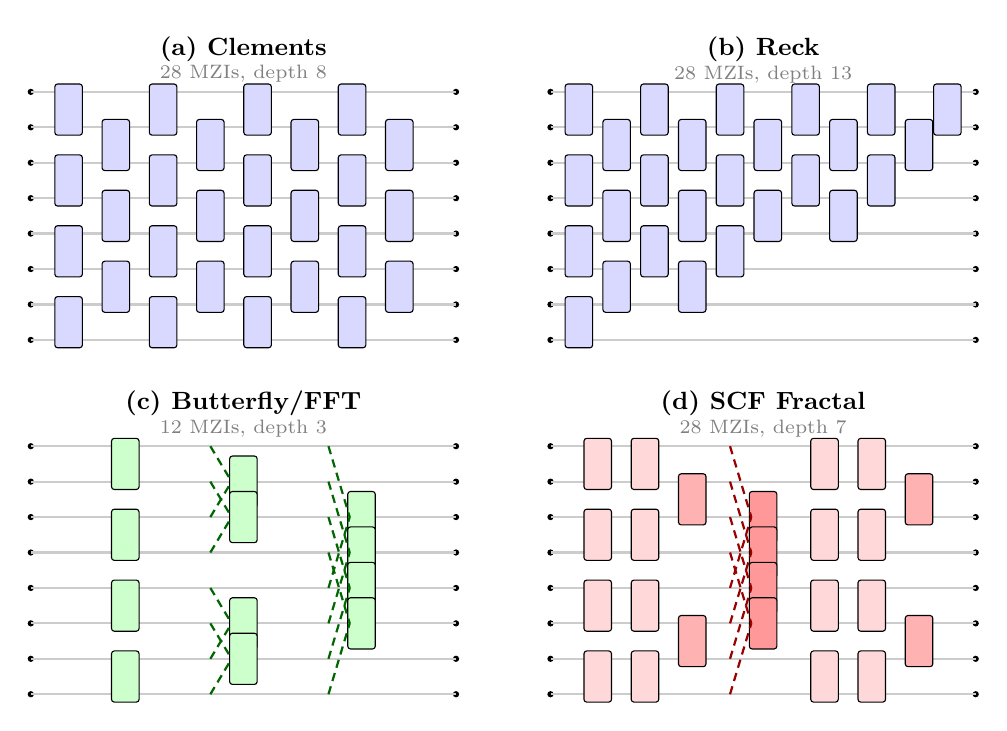
\begin{tikzpicture}[
    mzi/.style={draw, fill=blue!15, minimum width=0.35cm, minimum height=0.65cm, inner sep=0pt, rounded corners=1pt},
    port/.style={circle, fill=black, inner sep=0.8pt},
    waveguide/.style={thick, black!70},
    x=0.60cm, y=0.45cm
]

% ── Clements (N=8) ──
\begin{scope}[shift={(0,0)}]
\node[font=\bfseries\small] at (4.5, 1.2) {(a) Clements};
\node[font=\scriptsize, text=gray] at (4.5, 0.5) {28 MZIs, depth 8};

\foreach \p in {0,...,7} {
    \node[port] at (0, -\p) {};
    \node[port] at (9, -\p) {};
    \draw[waveguide, black!20] (0, -\p) -- (9, -\p);
}

% 8 columns, alternating even/odd
% Col 0,2,4,6 (even): pairs (0,1),(2,3),(4,5),(6,7)
% Col 1,3,5,7 (odd): pairs (1,2),(3,4),(5,6)
\foreach \col in {0,2,4,6} {
    \foreach \base in {0,2,4,6} {
        \pgfmathtruncatemacro{\top}{\base}
        \pgfmathtruncatemacro{\bot}{\base+1}
        \pgfmathsetmacro{\xp}{\col+0.8}
        \node[mzi] at (\xp, {-(\top+\bot)/2}) {};
    }
}
\foreach \col in {1,3,5,7} {
    \foreach \base in {1,3,5} {
        \pgfmathtruncatemacro{\top}{\base}
        \pgfmathtruncatemacro{\bot}{\base+1}
        \pgfmathsetmacro{\xp}{\col+0.8}
        \node[mzi] at (\xp, {-(\top+\bot)/2}) {};
    }
}
\end{scope}

% ── Reck (N=8) ──
\begin{scope}[shift={(11,0)}]
\node[font=\bfseries\small] at (4.5, 1.2) {(b) Reck};
\node[font=\scriptsize, text=gray] at (4.5, 0.5) {28 MZIs, depth 13};

\foreach \p in {0,...,7} {
    \node[port] at (0, -\p) {};
    \node[port] at (9, -\p) {};
    \draw[waveguide, black!20] (0, -\p) -- (9, -\p);
}

% Triangular pattern - decreasing MZIs per column
% Column positions spread across width
\node[mzi] at (0.6, -0.5) {};
\node[mzi] at (0.6, -2.5) {};
\node[mzi] at (0.6, -4.5) {};
\node[mzi] at (0.6, -6.5) {};

\node[mzi] at (1.4, -1.5) {};
\node[mzi] at (1.4, -3.5) {};
\node[mzi] at (1.4, -5.5) {};

\node[mzi] at (2.2, -0.5) {};
\node[mzi] at (2.2, -2.5) {};
\node[mzi] at (2.2, -4.5) {};

\node[mzi] at (3.0, -1.5) {};
\node[mzi] at (3.0, -3.5) {};
\node[mzi] at (3.0, -5.5) {};

\node[mzi] at (3.8, -0.5) {};
\node[mzi] at (3.8, -2.5) {};
\node[mzi] at (3.8, -4.5) {};

\node[mzi] at (4.6, -1.5) {};
\node[mzi] at (4.6, -3.5) {};

\node[mzi] at (5.4, -0.5) {};
\node[mzi] at (5.4, -2.5) {};

\node[mzi] at (6.2, -1.5) {};
\node[mzi] at (6.2, -3.5) {};

\node[mzi] at (7.0, -0.5) {};
\node[mzi] at (7.0, -2.5) {};

\node[mzi] at (7.8, -1.5) {};

\node[mzi] at (8.4, -0.5) {};
\end{scope}

% ── Butterfly (N=8) ──
\begin{scope}[shift={(0,-10)}]
\node[font=\bfseries\small] at (4.5, 1.2) {(c) Butterfly/FFT};
\node[font=\scriptsize, text=gray] at (4.5, 0.5) {12 MZIs, depth 3};

\foreach \p in {0,...,7} {
    \node[port] at (0, -\p) {};
    \node[port] at (9, -\p) {};
    \draw[waveguide, black!20] (0, -\p) -- (9, -\p);
}

% Stage 0: stride 1 — pairs (0,1),(2,3),(4,5),(6,7)
\foreach \base in {0,2,4,6} {
    \pgfmathtruncatemacro{\bot}{\base+1}
    \node[mzi, fill=green!20] at (2, {-(\base+\bot)/2}) {};
}
% Stage 1: stride 2 — pairs (0,2),(1,3),(4,6),(5,7)
\node[mzi, fill=green!20] at (4.5, -1) {};
\draw[waveguide, green!40!black, densely dashed] (3.8, 0) -- (4.25, -1) (3.8, -2) -- (4.25, -1);
\node[mzi, fill=green!20] at (4.5, -2) {};
\draw[waveguide, green!40!black, densely dashed] (3.8, -1) -- (4.25, -2) (3.8, -3) -- (4.25, -2);
\node[mzi, fill=green!20] at (4.5, -5) {};
\draw[waveguide, green!40!black, densely dashed] (3.8, -4) -- (4.25, -5) (3.8, -6) -- (4.25, -5);
\node[mzi, fill=green!20] at (4.5, -6) {};
\draw[waveguide, green!40!black, densely dashed] (3.8, -5) -- (4.25, -6) (3.8, -7) -- (4.25, -6);

% Stage 2: stride 4 — pairs (0,4),(1,5),(2,6),(3,7)
\node[mzi, fill=green!20] at (7, -2) {};
\draw[waveguide, green!40!black, densely dashed] (6.3, 0) -- (6.75, -2) (6.3, -4) -- (6.75, -2);
\node[mzi, fill=green!20] at (7, -3) {};
\draw[waveguide, green!40!black, densely dashed] (6.3, -1) -- (6.75, -3) (6.3, -5) -- (6.75, -3);
\node[mzi, fill=green!20] at (7, -4) {};
\draw[waveguide, green!40!black, densely dashed] (6.3, -2) -- (6.75, -4) (6.3, -6) -- (6.75, -4);
\node[mzi, fill=green!20] at (7, -5) {};
\draw[waveguide, green!40!black, densely dashed] (6.3, -3) -- (6.75, -5) (6.3, -7) -- (6.75, -5);
\end{scope}

% ── SCF Fractal (N=8) ──
\begin{scope}[shift={(11,-10)}]
\node[font=\bfseries\small] at (4.5, 1.2) {(d) SCF Fractal};
\node[font=\scriptsize, text=gray] at (4.5, 0.5) {28 MZIs, depth 7};

\foreach \p in {0,...,7} {
    \node[port] at (0, -\p) {};
    \node[port] at (9, -\p) {};
    \draw[waveguide, black!20] (0, -\p) -- (9, -\p);
}

% SCF: recursive structure - sub-blocks then mixing then sub-blocks
% Left sub-block: top 4 ports, bottom 4 ports (parallel)
\node[mzi, fill=red!15] at (1.0, -0.5) {};
\node[mzi, fill=red!15] at (1.0, -2.5) {};
\node[mzi, fill=red!15] at (1.0, -4.5) {};
\node[mzi, fill=red!15] at (1.0, -6.5) {};

% Second level sub-blocks
\node[mzi, fill=red!15] at (2.0, -0.5) {};
\node[mzi, fill=red!15] at (2.0, -2.5) {};
\node[mzi, fill=red!15] at (2.0, -4.5) {};
\node[mzi, fill=red!15] at (2.0, -6.5) {};

% Sub-sub mixing
\node[mzi, fill=red!30] at (3.0, -1.5) {};
\node[mzi, fill=red!30] at (3.0, -5.5) {};

% Mixing layer: connect top[i] with bot[i]
\node[mzi, fill=red!40] at (4.5, -2) {};
\draw[waveguide, red!60!black, densely dashed] (3.8, 0) -- (4.25, -2) (3.8, -4) -- (4.25, -2);
\node[mzi, fill=red!40] at (4.5, -3) {};
\draw[waveguide, red!60!black, densely dashed] (3.8, -1) -- (4.25, -3) (3.8, -5) -- (4.25, -3);
\node[mzi, fill=red!40] at (4.5, -4) {};
\draw[waveguide, red!60!black, densely dashed] (3.8, -2) -- (4.25, -4) (3.8, -6) -- (4.25, -4);
\node[mzi, fill=red!40] at (4.5, -5) {};
\draw[waveguide, red!60!black, densely dashed] (3.8, -3) -- (4.25, -5) (3.8, -7) -- (4.25, -5);

% Right sub-blocks (mirror)
\node[mzi, fill=red!15] at (5.8, -0.5) {};
\node[mzi, fill=red!15] at (5.8, -2.5) {};
\node[mzi, fill=red!15] at (5.8, -4.5) {};
\node[mzi, fill=red!15] at (5.8, -6.5) {};

\node[mzi, fill=red!15] at (6.8, -0.5) {};
\node[mzi, fill=red!15] at (6.8, -2.5) {};
\node[mzi, fill=red!15] at (6.8, -4.5) {};
\node[mzi, fill=red!15] at (6.8, -6.5) {};

\node[mzi, fill=red!30] at (7.8, -1.5) {};
\node[mzi, fill=red!30] at (7.8, -5.5) {};
\end{scope}

\end{tikzpicture}
\caption{Schematic wiring diagrams for the four MZI mesh topologies at $N{=}8$. Each small rectangle represents one MZI operating on a pair of waveguides. Dashed lines indicate non-adjacent port connections requiring waveguide crossings. (a)~Clements: rectangular, 28 MZIs, depth~8. (b)~Reck: triangular, 28~MZIs, depth~13. (c)~Butterfly: FFT pattern, 12~MZIs, depth~3. (d)~SCF~Fractal: recursive CS decomposition, 28~MZIs, depth~7; shading indicates recursion level.}
\label{fig:schematics}
\end{figure*}


\subsection{Network architecture}

Each PNN consists of a single photonic mesh layer followed by photodetection and an electronic classifier (linear layer with 64 hidden units, ReLU activation, then a classification head).
Using a single photonic layer isolates the topology effect from multi-layer interactions.
Inputs are PCA-reduced to $N$ dimensions and normalized to $[0,1]$ for optical encoding.
Training uses Adam optimization for 100 epochs (vowel) or 15--30 epochs (Fashion-MNIST, which has ${\sim}100\times$ more training samples).


\subsection{Evaluation protocol}

Models are evaluated at seven phase noise levels: $\sigma \in \{0, 0.01, 0.02, 0.05, 0.1, 0.15, 0.2\}$\,rad.
For $\sigma > 0$, we run 30 Monte Carlo trials and report mean accuracy and standard deviation.
The \textit{robustness ratio} is defined as the mean accuracy at $\sigma{=}0.2$\,rad divided by the clean accuracy ($\sigma{=}0$).
\textit{Hardware cost} is defined as $\text{MZI count} \times \text{optical depth}$, a proxy for chip area and worst-case latency.
This composite metric is a simplification; MZI count and optical depth have distinct physical implications (chip area versus accumulated loss).
We verified that topology rankings are consistent when these axes are analyzed separately.
Pareto optimality identifies non-dominated points across the accuracy--cost plane.


\subsection{Datasets}

\textbf{Deterding vowel}~\cite{shen2017}: 11 classes, 10 features, ${\sim}550$ samples. The standard PNN benchmark since Shen~\textit{et al.}; included for comparability with prior work.

\textbf{Fashion-MNIST}~\cite{xiao2017}: 10 classes, 784 features PCA-reduced to $N$, 60{,}000 training / 10{,}000 test samples. A harder task that tests whether topology advantages persist with more data and more classes.


%% ================================================================
\section{Results}
\label{sec:results}

\subsection{Pareto front analysis}

Figure~\ref{fig:pareto} shows accuracy versus hardware cost for all topologies and mesh sizes on both datasets, at $\sigma{=}0$ (clean) and $\sigma{=}0.1$\,rad.
Table~\ref{tab:n16results} reports the $N{=}16$ results in detail.

\begin{table}[b]
\caption{Performance at $N{=}16$ on vowel dataset (0.2\,dB/MZI loss), averaged over 4 training runs with different random seeds. Robustness ratio defined as accuracy at $\sigma{=}0.2$ divided by clean accuracy.}
\label{tab:n16results}
\begin{ruledtabular}
\begin{tabular}{lccccc}
Topology & MZIs & Depth & Cost & Acc.\,(\%) & Robust.\ \\
\hline
Clements    & 120 & 16 & 1920 & $82.7 \pm 0.9$ & $0.208 \pm 0.004$ \\
Reck        & 120 & 29 & 3480 & $83.6 \pm 2.3$ & $0.252 \pm 0.029$ \\
Butterfly   &  32 &  4 &  128 & $84.3 \pm 1.7$ & $0.377 \pm 0.032$ \\
SCF Fractal & 120 & 15 & 1800 & $84.7 \pm 0.9$ & $0.210 \pm 0.013$ \\
\end{tabular}
\end{ruledtabular}
\end{table}

Butterfly occupies the Pareto-optimal lower-left region (low cost, competitive accuracy) at every noise level.
At $N{=}16$ on vowel, butterfly achieves $84.3 \pm 1.7$\% accuracy at hardware cost 128, compared to Clements at $82.7 \pm 0.9$\% and cost 1920, representing a 15$\times$ cost reduction with comparable accuracy.
On Fashion-MNIST (single runs), the pattern is similar: butterfly reaches 79.7\% at cost~128 versus Clements at 78.0\% at cost~1920.
At $N{=}32$ the gap widens further: butterfly achieves 85.5\% at cost 400, versus Clements at 82.2\% at cost 15{,}872 (40$\times$).

Among universal topologies, Reck achieves the highest mean clean accuracy at $N{=}16$ on vowel ($83.6 \pm 2.3$\%) but at the highest hardware cost (3480).
SCF Fractal ($84.7 \pm 0.9$\%) slightly outperforms Clements ($82.7 \pm 0.9$\%) at similar depth, but both sit far from the Pareto front due to their high MZI count.

\begin{figure*}[t]
\centering
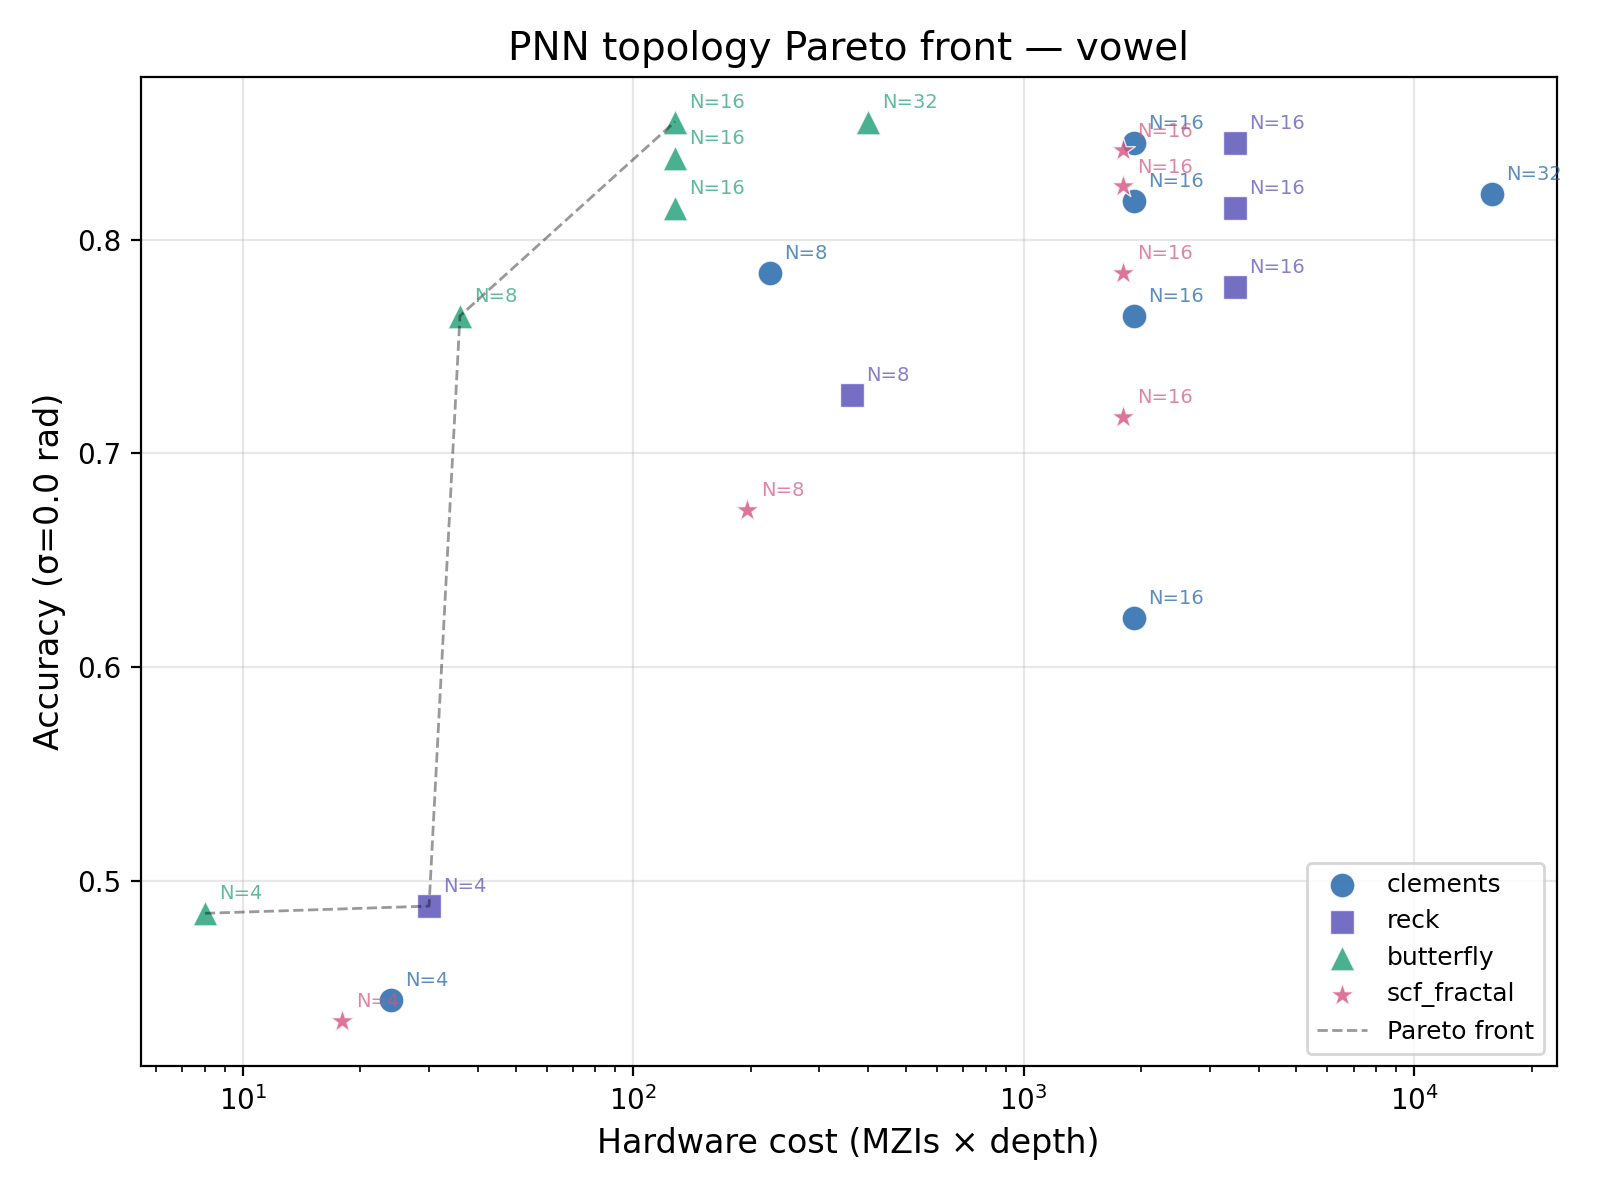
\includegraphics[width=0.48\textwidth]{results/figures/pareto_sigma0.00_vowel.png}%
\hfill
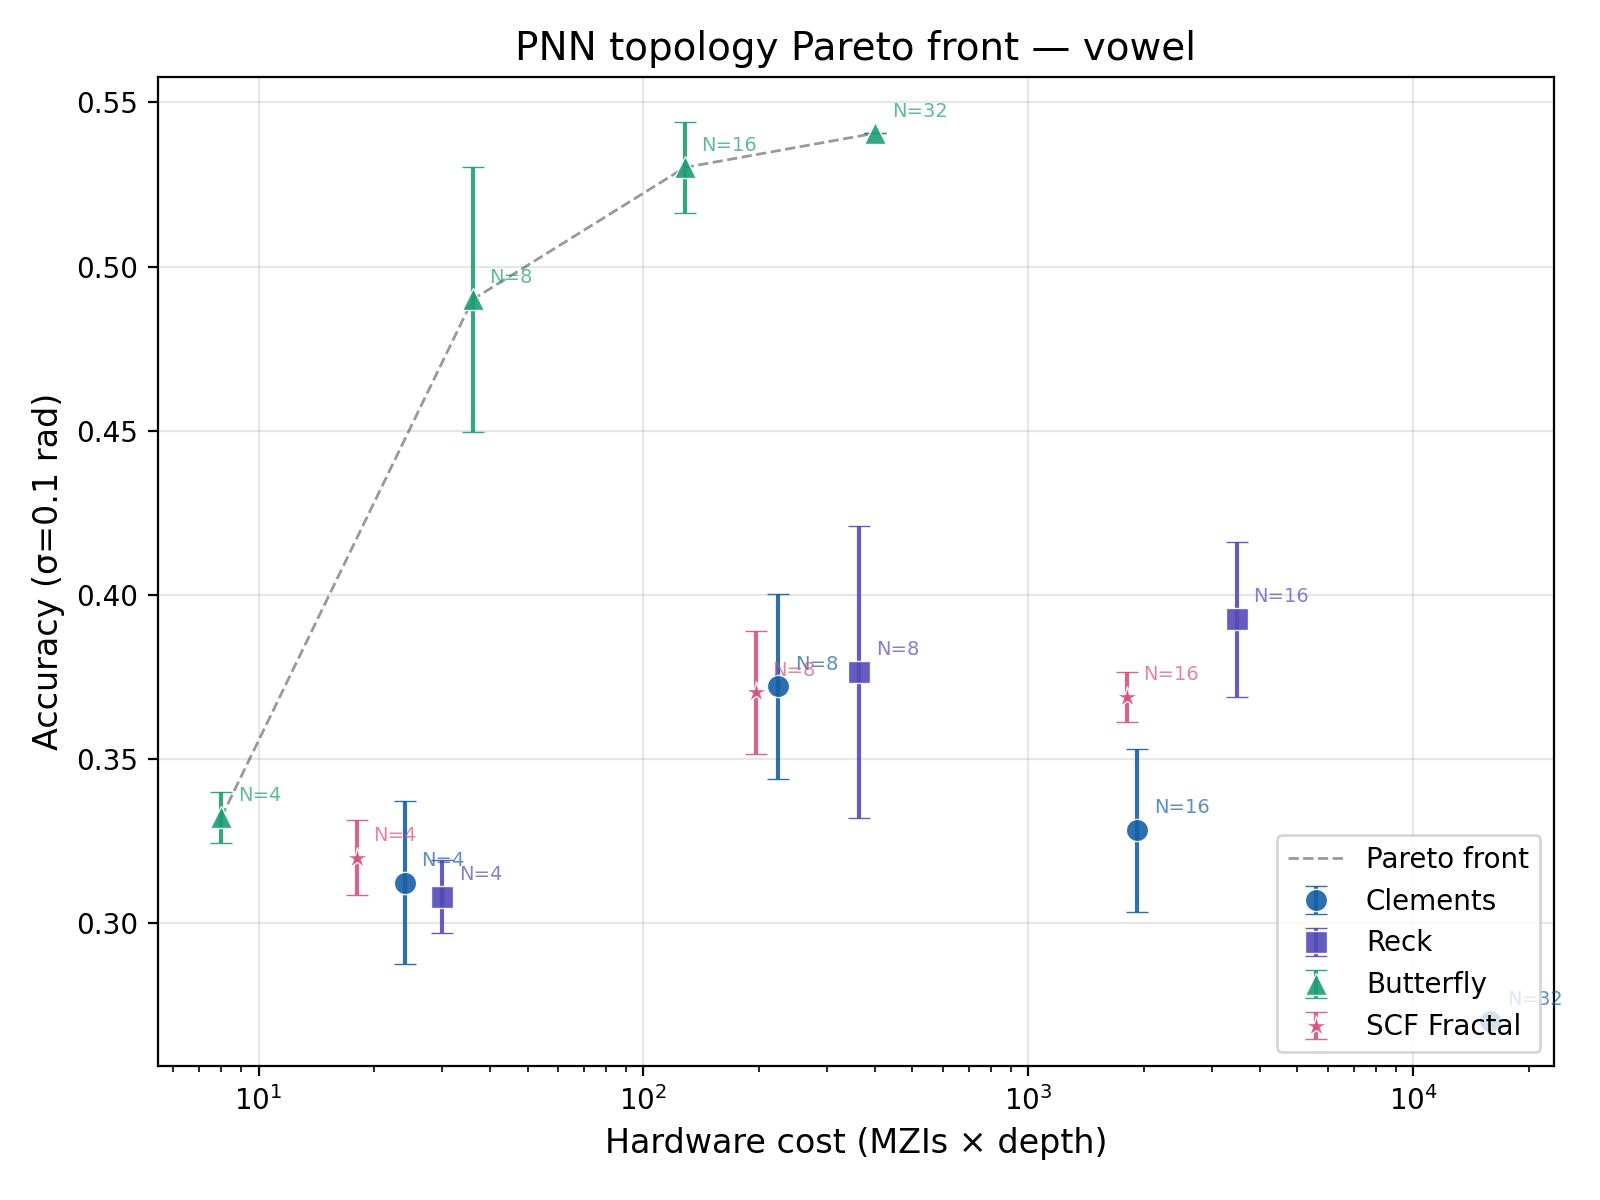
\includegraphics[width=0.48\textwidth]{results/figures/pareto_sigma0.10_vowel.png}
\\[2pt]
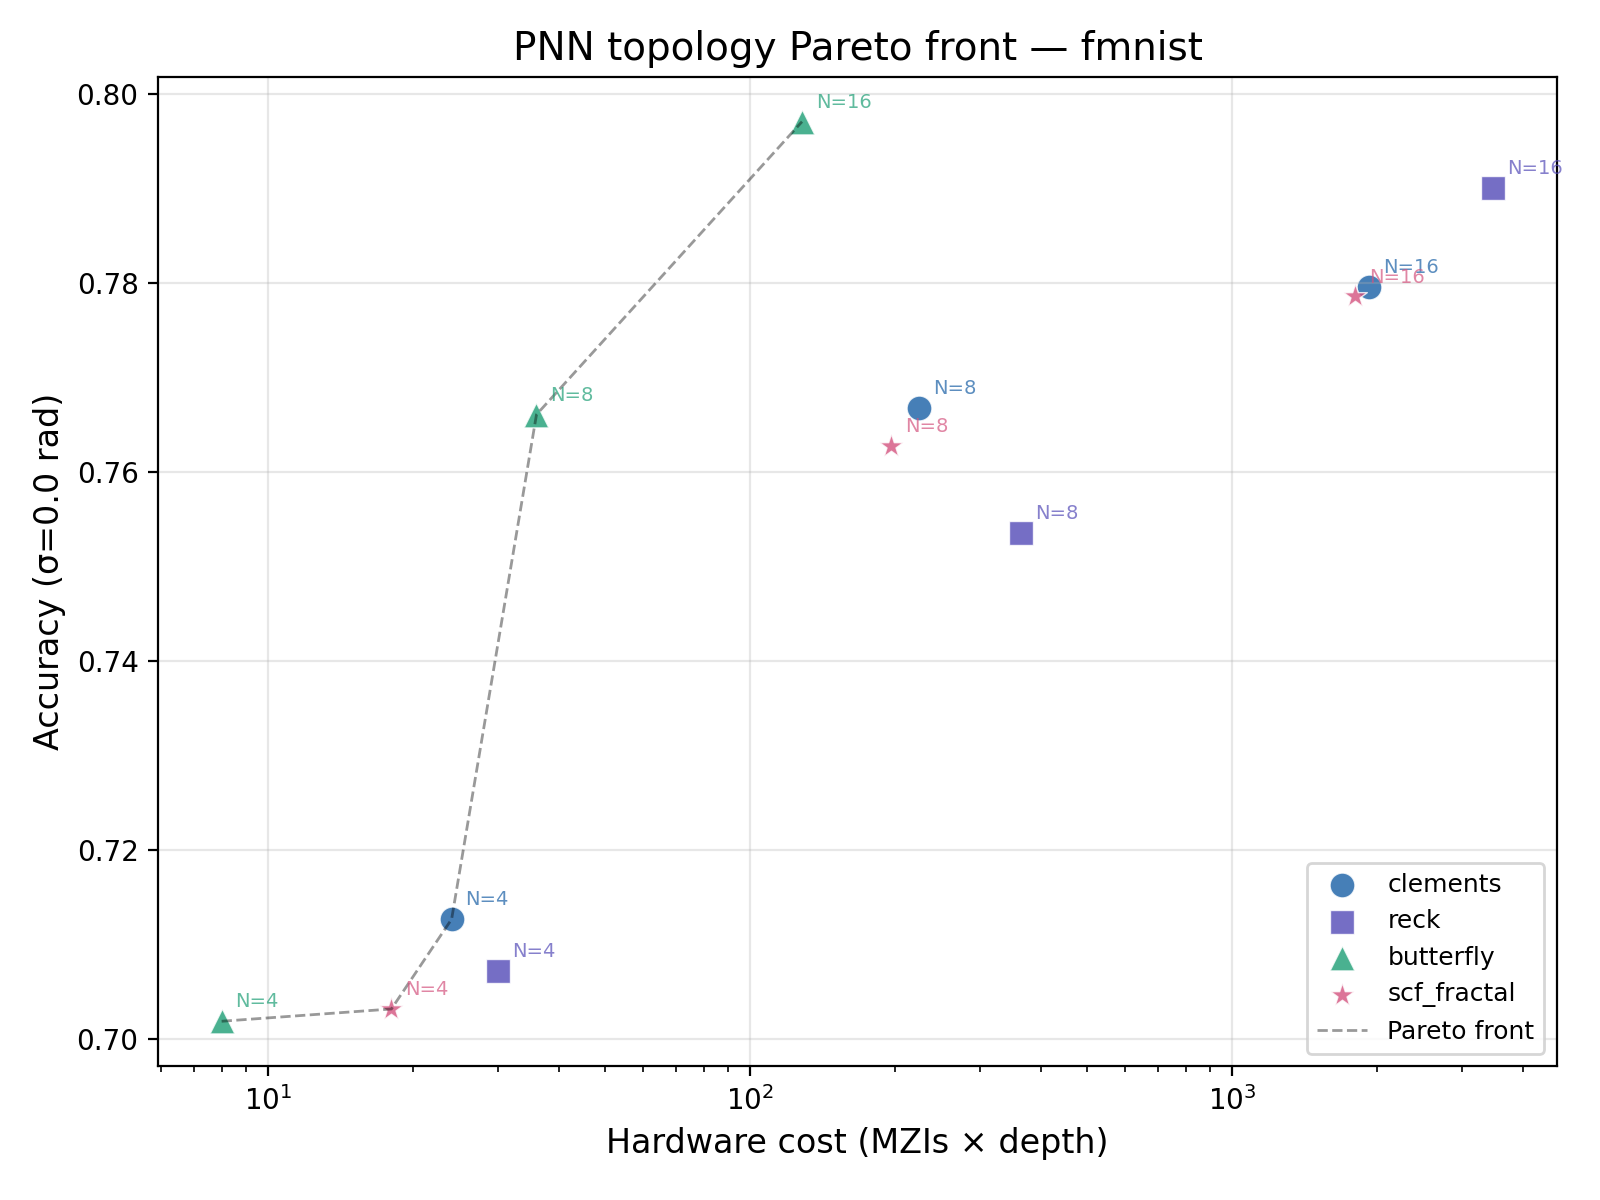
\includegraphics[width=0.48\textwidth]{results/figures/pareto_sigma0.00_fmnist.png}%
\hfill
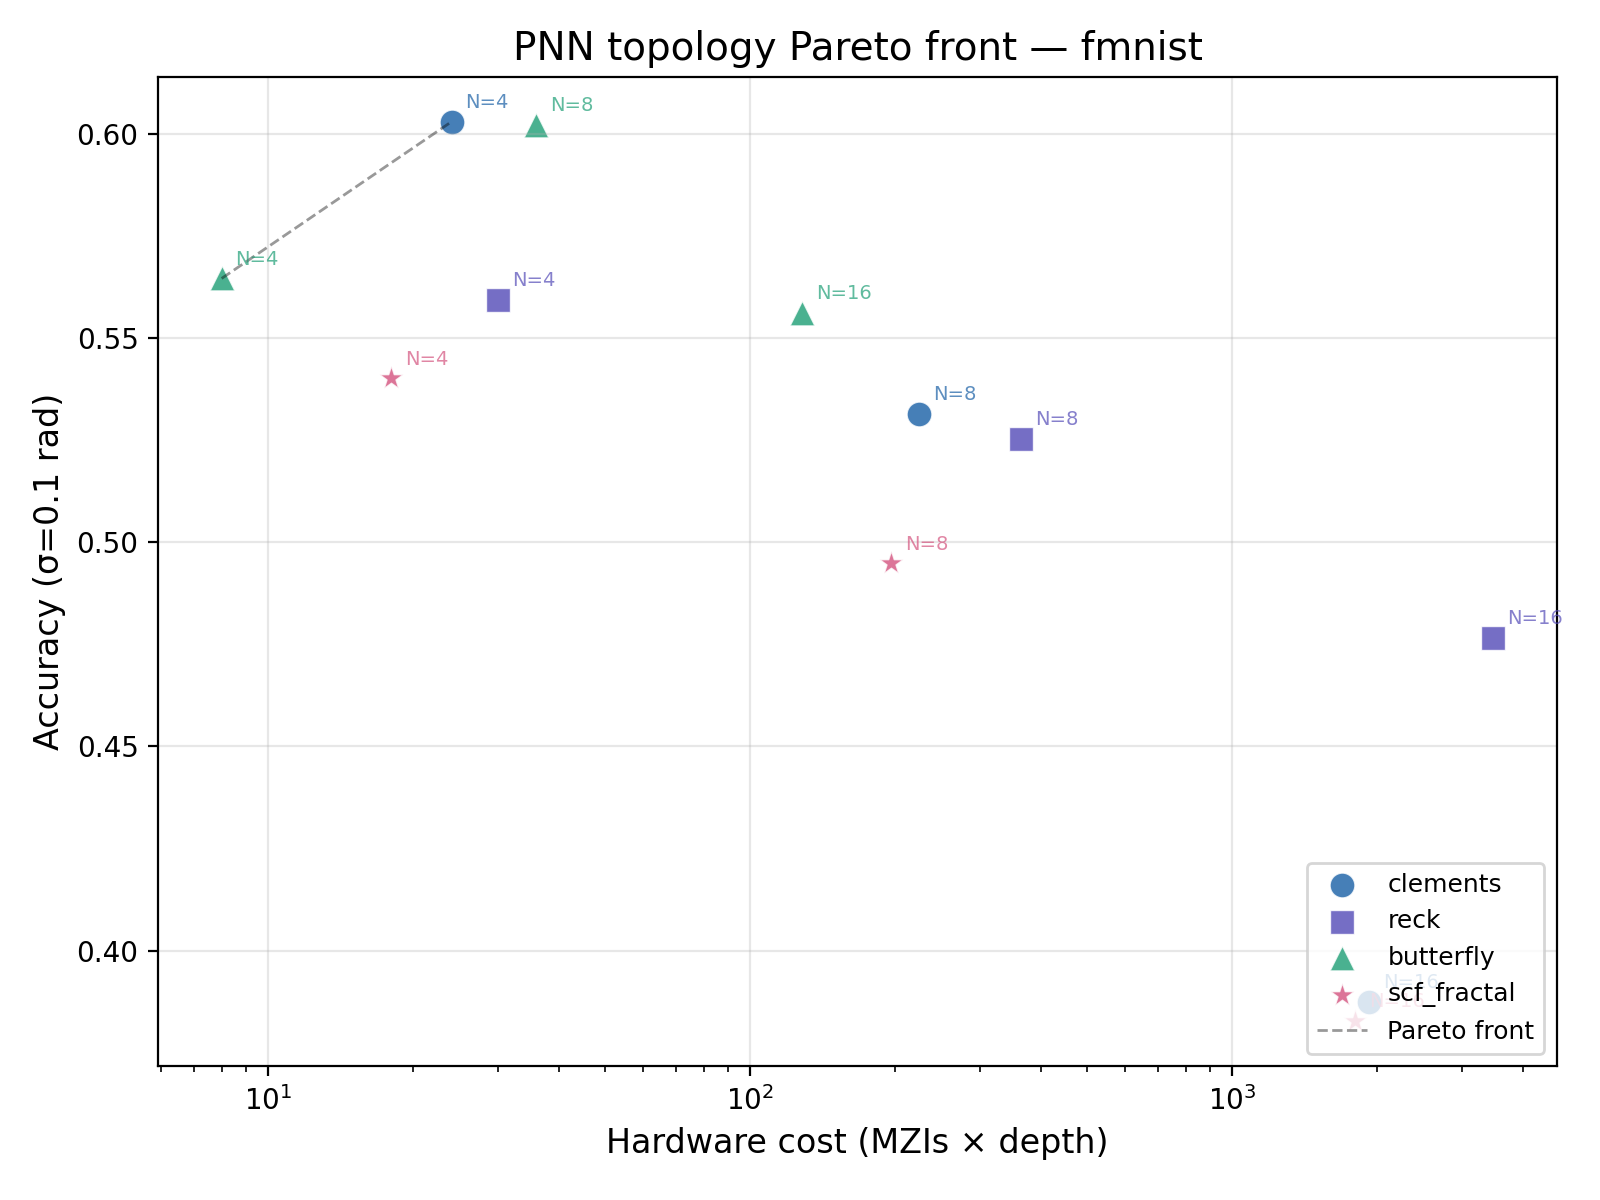
\includegraphics[width=0.48\textwidth]{results/figures/pareto_sigma0.10_fmnist.png}
\caption{Pareto front: accuracy versus hardware cost (MZIs\,$\times$\,depth) for all topologies and mesh sizes. Left column: clean ($\sigma{=}0$). Right column: noisy ($\sigma{=}0.1$\,rad). Top row: vowel dataset (mean $\pm$ std over 4 seeds). Bottom row: Fashion-MNIST (single runs). Dashed line indicates the Pareto front computed from mean values.}
\label{fig:pareto}
\end{figure*}


\subsection{Robustness versus depth}

Figure~\ref{fig:robustness} shows accuracy versus phase noise $\sigma$ for all topologies at $N{=}16$.
There is a clear relationship between optical depth and noise sensitivity, though not perfectly monotonic.
Butterfly (depth~4) retains $37.7 \pm 3.2$\% of its clean accuracy at $\sigma{=}0.2$ on vowel (averaged over 4 seeds) and 43\% on Fashion-MNIST.
Clements (depth~16) and SCF Fractal (depth~15) retain only $20.8 \pm 0.4$\% and $21.0 \pm 1.3$\%, respectively.

Reck presents a notable result: despite having the deepest topology (depth~29), it achieves robustness of $0.252 \pm 0.029$, consistently better than Clements ($0.208 \pm 0.004$) across all 4 training seeds.
We attribute this to Reck's triangular structure, in which some output ports are reached through significantly fewer MZIs than the maximum depth, effectively creating a distribution of path lengths rather than a uniform depth.
This suggests that \emph{maximum depth} alone does not fully determine robustness; the distribution of path lengths matters.

SCF Fractal's theoretical $O(N\sigma^4)$ error scaling advantage~\cite{basani2023} is not apparent in our results.
At $N{=}16$, SCF (depth~15) and Clements (depth~16) show essentially identical robustness ($0.210 \pm 0.013$ vs.\ $0.208 \pm 0.004$).
The $\sigma^4$ advantage likely manifests at very small $\sigma$ where the depth-driven $\sigma^2$ effect does not yet dominate; at the noise levels relevant to current foundries ($\sigma > 0.01$), depth is the primary determinant.

\begin{figure}[t]
\centering
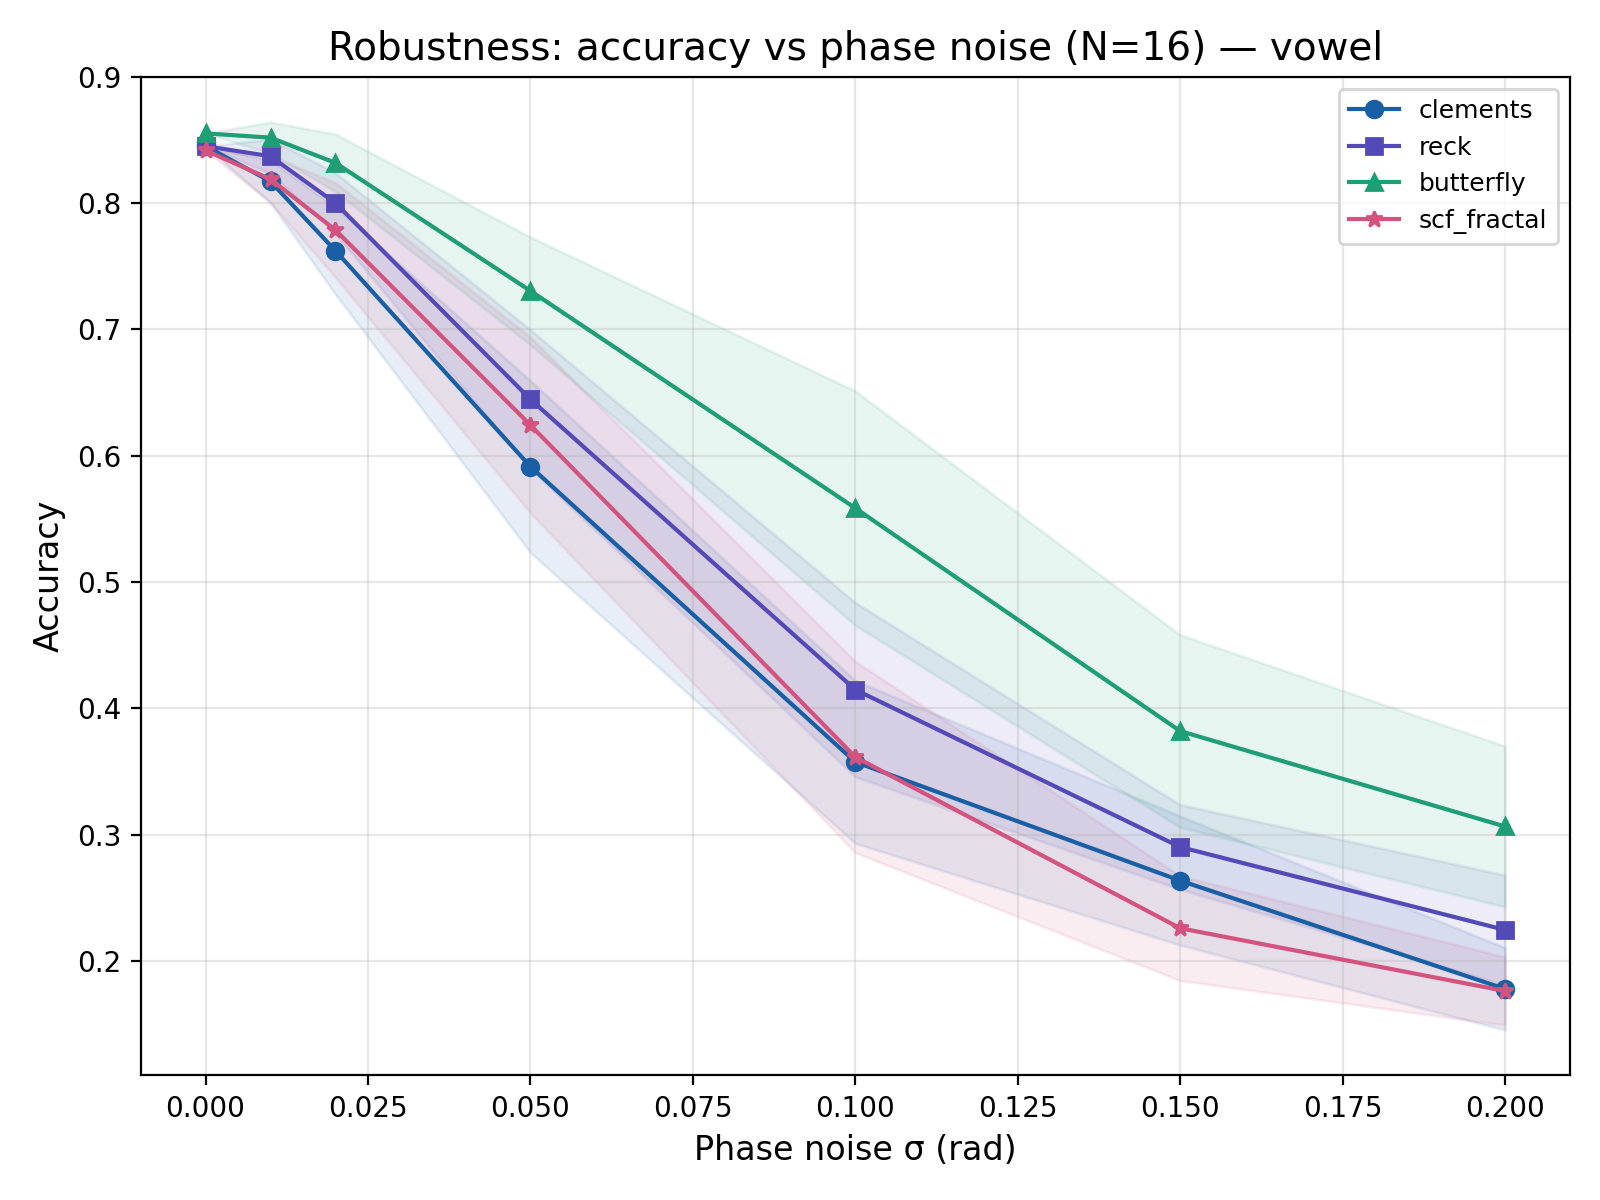
\includegraphics[width=0.9\columnwidth]{results/figures/robustness_N16_vowel.png}
\caption{Accuracy versus phase noise $\sigma$ for all topologies at $N{=}16$ on vowel. Shaded regions show $\pm 1$ standard deviation over 30 Monte Carlo trials. Butterfly's shallow depth (4 layers) provides consistently superior noise tolerance. Fashion-MNIST results show the same pattern (butterfly retains 43\% at $\sigma{=}0.2$ versus 24\% for Clements).}
\label{fig:robustness}
\end{figure}


\subsection{Insertion loss sensitivity}

Table~\ref{tab:loss} shows the effect of increasing per-MZI insertion loss from 0.2 to 0.5\,dB at $N{=}16$ on vowel, averaged over 4 random seeds.
Butterfly is the most loss-tolerant topology: its mean clean accuracy drops only 2.6\,pp from 0.2 to 0.5\,dB/MZI (from $84.3 \pm 1.7$\% to $81.7 \pm 0.4$\%), because signals traverse only 4 MZIs.
Clements drops 4.6\,pp (from $82.7 \pm 0.9$\% to $78.1 \pm 1.5$\%) and SCF Fractal drops 5.0\,pp, as their signals traverse 15--16 MZIs.
The robustness ratio remains largely stable across loss levels for all topologies, indicating that the topology ranking does not change with foundry quality; butterfly's advantage simply grows in magnitude.

\begin{table}[t]
\caption{Insertion loss sensitivity at $N{=}16$, vowel dataset, averaged over 4 random seeds. Clean accuracy (\%) and robustness ratio at three loss levels. Uncertainties are one standard deviation.}
\label{tab:loss}
\begin{ruledtabular}
\begin{tabular}{lcccccc}
 & \multicolumn{2}{c}{0.2\,dB} & \multicolumn{2}{c}{0.3\,dB} & \multicolumn{2}{c}{0.5\,dB} \\
\cmidrule(lr){2-3}\cmidrule(lr){4-5}\cmidrule(lr){6-7}
Topology & Acc & Rob & Acc & Rob & Acc & Rob \\
\hline
Clements    & $82.7{\pm}0.9$ & $0.21$ & $81.7{\pm}2.7$ & $0.22$ & $78.1{\pm}1.5$ & $0.23$ \\
Reck        & $83.6{\pm}2.3$ & $0.25$ & $80.6{\pm}1.6$ & $0.28$ & $79.3{\pm}2.7$ & $0.30$ \\
Butterfly   & $84.3{\pm}1.7$ & $0.38$ & $84.5{\pm}1.0$ & $0.38$ & $81.7{\pm}0.4$ & $0.40$ \\
SCF Fractal & $84.7{\pm}0.9$ & $0.21$ & $82.0{\pm}0.4$ & $0.23$ & $79.7{\pm}0.9$ & $0.22$ \\
\end{tabular}
\end{ruledtabular}
\end{table}


\subsection{Noise-aware training}

Table~\ref{tab:noiseaware} compares standard and noise-aware training for Clements and SCF Fractal at $N{=}16$ on vowel, both averaged over 4 random seeds.
Noise-aware training (injecting $\sigma{=}0.05$ during training) improves robustness ratios: +35\% relative for Clements (from $0.208 \pm 0.004$ to $0.281 \pm 0.016$), +25\% for SCF Fractal (from $0.210 \pm 0.013$ to $0.262 \pm 0.006$).
However, this comes at a cost in clean accuracy: $-$16.9\,pp for Clements (from $82.7 \pm 0.9$\% to $65.8 \pm 3.3$\%) and $-$13.4\,pp for SCF Fractal (from $84.7 \pm 0.9$\% to $71.3 \pm 1.9$\%).

Notably, butterfly \emph{without} noise-aware training achieves better robustness ($0.377 \pm 0.032$) than Clements \emph{with} it ($0.281 \pm 0.016$).
In this regime, topology choice has a larger effect on robustness than training strategy.

\begin{table}[t]
\caption{Standard versus noise-aware training at $N{=}16$, vowel, 0.2\,dB/MZI. All values are mean $\pm$ std over 4 random seeds. Noise-aware training injects $\sigma{=}0.05$ during training.}
\label{tab:noiseaware}
\begin{ruledtabular}
\begin{tabular}{lccccc}
 & \multicolumn{2}{c}{Standard} & \multicolumn{2}{c}{Noise-aware} \\
\cmidrule(lr){2-3}\cmidrule(lr){4-5}
Topology & Acc\,(\%) & Rob & Acc\,(\%) & Rob \\
\hline
Clements    & $82.7 \pm 0.9$ & $0.208 \pm 0.004$ & $65.8 \pm 3.3$ & $0.281 \pm 0.016$ \\
SCF Fractal & $84.7 \pm 0.9$ & $0.210 \pm 0.013$ & $71.3 \pm 1.9$ & $0.262 \pm 0.006$ \\
\hline
Butterfly (std) & $84.3 \pm 1.7$ & $0.377 \pm 0.032$ & \multicolumn{2}{c}{---} \\
\end{tabular}
\end{ruledtabular}
\end{table}


\subsection{Scaling}

Figure~\ref{fig:scaling} shows classification accuracy versus mesh size $N$ for each topology.
All topologies improve monotonically with $N$, reflecting both increased parameter count and better PCA input representation.
Butterfly matches or exceeds universal topologies at $N \geq 8$ despite its non-universality: at $N{=}32$, butterfly (85.5\%) outperforms Clements (82.2\%) while the hardware cost gap widens from $15\times$ at $N{=}16$ to $40\times$ at $N{=}32$, following the $O(N^2)$ versus $O(N\log N)$ scaling.

\begin{figure}[t]
\centering
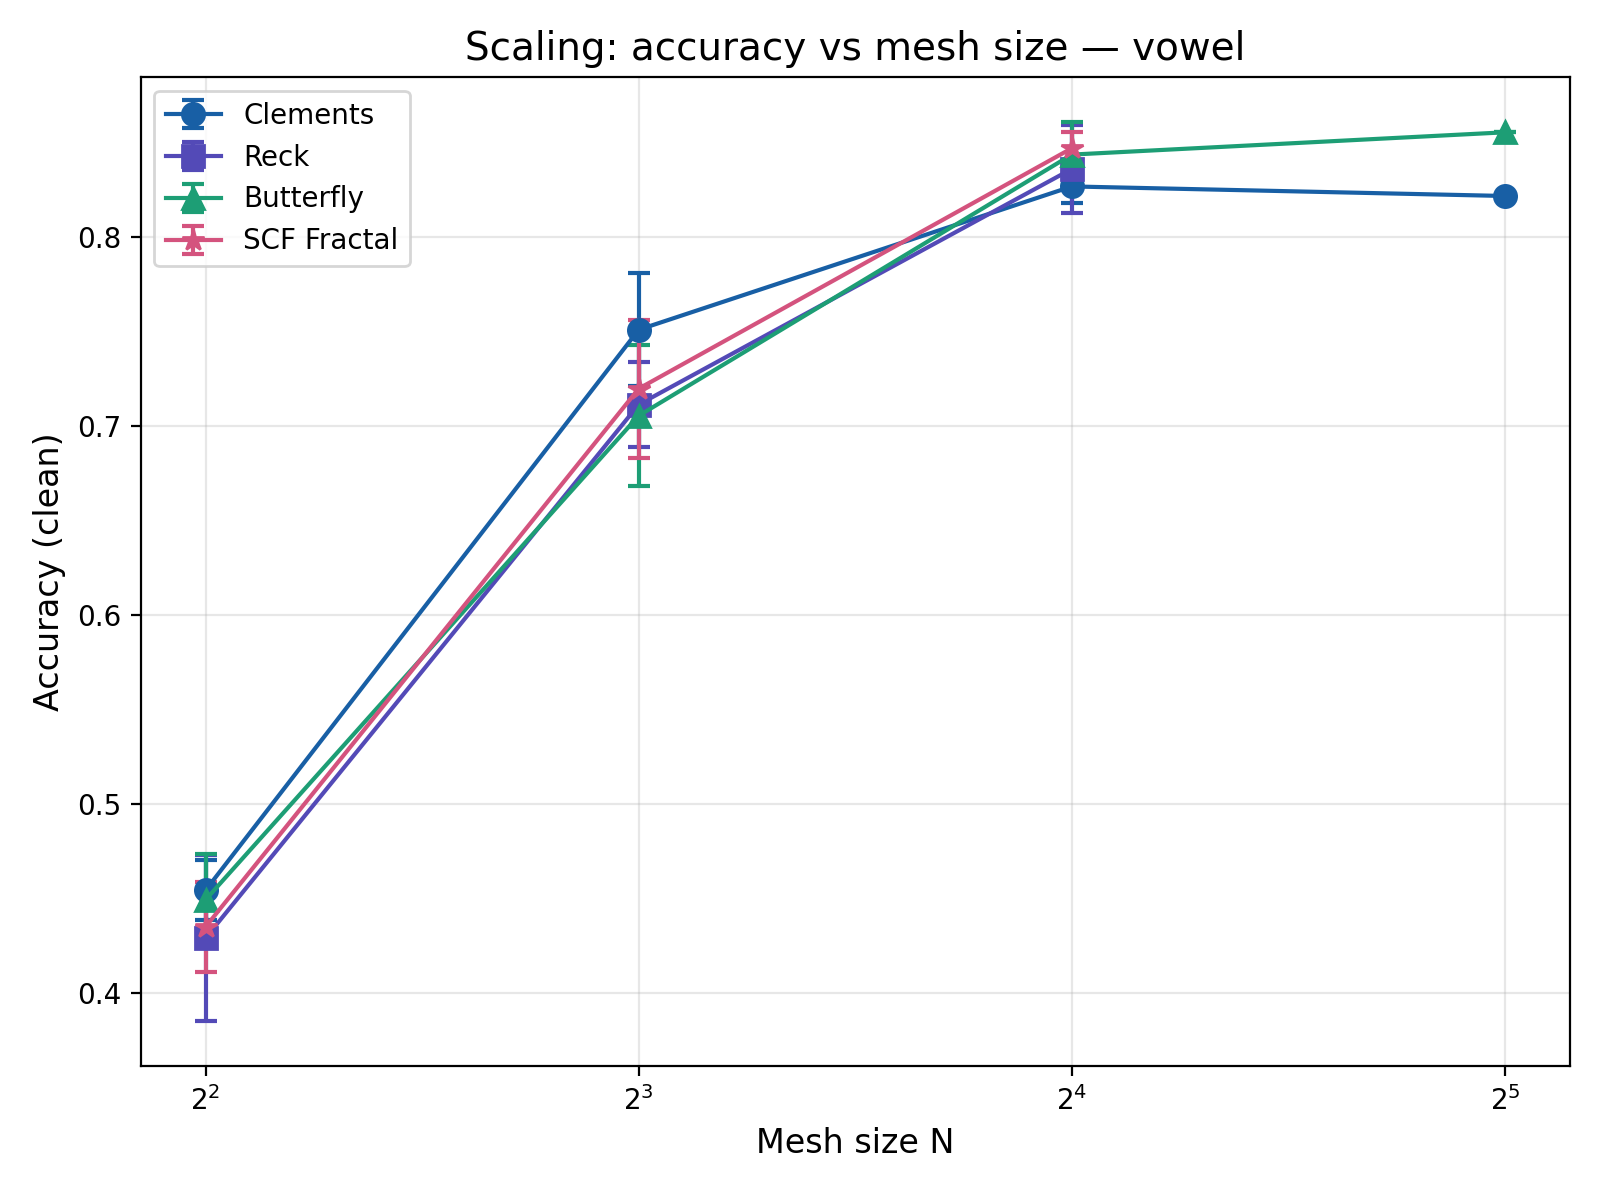
\includegraphics[width=0.9\columnwidth]{results/figures/scaling_sigma0.00_vowel.png}
\caption{Clean accuracy versus mesh size $N$ on vowel (mean $\pm$ std over 4 seeds). $N{=}32$ was run for Clements and butterfly only.}
\label{fig:scaling}
\end{figure}


%% ================================================================
\section{Discussion}
\label{sec:discussion}

\textit{Why butterfly wins, and when it might not.}
Butterfly's Pareto dominance derives from its $O(\log N)$ depth.
Depth drives both phase noise accumulation and insertion loss, making it the primary determinant of robustness in realistic photonic systems.
However, butterfly implements only a strict subgroup of $U(N)$: for applications requiring arbitrary unitary transformations (quantum computing, optical channel estimation), universal topologies like Clements remain necessary.
Our results show that classification does not require universality: the network learns effective transformations within the butterfly subgroup at every tested scale.

\textit{What we did not model.}
Our simulations have several simplifications that could affect the relative topology ranking:
\begin{itemize}
\item \emph{Waveguide crossing loss.} Butterfly requires physical waveguide crossings for non-adjacent port connections (visible as dashed lines in Fig.~\ref{fig:schematics}c,d). At ${\sim}0.02$\,dB per crossing~\cite{shafiee2023}, this could partially offset butterfly's depth advantage. Quantifying this requires layout-level analysis specific to the target foundry and technology node.
\item \emph{Wavelength dependence.} MZI splitting ratios vary with wavelength. This affects all topologies but penalizes deeper meshes more, likely reinforcing butterfly's advantage, though we have not modeled this.
\item \emph{Coupler imbalance.} We model phase errors only. Directional coupler splitting ratio errors are an additional impairment that may affect topologies differently~\cite{marchesin2025}.
\item \emph{Diamond and braid topologies.} Their path-balancing properties~\cite{shokraneh2020,marchesin2025} could improve robustness by equalizing loss across all input--output paths. These are important comparisons that we leave for future work.
\end{itemize}

\textit{Practical recommendations.}
For chip designers choosing a topology for inference tasks: if the application is classification or regression, butterfly provides the best accuracy--cost--robustness tradeoff at all tested scales.
If universality is required, Clements is preferable to Reck (lower depth at same MZI count).
For lossy foundries ($> 0.3$\,dB/MZI), butterfly's advantage grows.
We recommend investing in topology selection before noise-aware training, as the former provides larger robustness gains without sacrificing clean accuracy.
These guidelines apply to the tested regime ($N \leq 32$, classification tasks); they may not hold at $N \geq 128$ or for tasks that fully exploit unitary expressiveness.

\textit{The benchmark framework.}
The framework is open-source and extensible: adding a topology requires implementing a single function that returns a list of MZI layers and port assignments.
Validated implementations of diamond, braid, and other emerging topologies would enable a more comprehensive comparison.


%% ================================================================
\section{Conclusion}
\label{sec:conclusion}

We compared four MZI mesh topologies under identical training, insertion loss, and phase noise conditions across 72 experiments.
Butterfly/FFT consistently occupies the Pareto front, achieving comparable classification accuracy to universal topologies at substantially lower hardware cost and with better noise robustness.
The advantage is driven by its $O(\log N)$ optical depth and grows with both mesh size and insertion loss.
In the tested regime, topology choice had a larger effect on robustness than noise-aware training.

Open questions remain: the impact of waveguide crossing loss on butterfly's advantage, whether diamond and braid topologies' path-balancing properties can challenge butterfly on robustness, and whether non-universality becomes a limitation at larger scales or for more complex tasks.
The framework and all experimental data are publicly available to facilitate these investigations.

\subsection*{Data availability}
The simulation framework, experiment logs, and all data needed to reproduce these results are available at \url{https://github.com/LTalandier/pnn-pareto-benchmark}.


%% ================================================================
\begin{acknowledgments}
The authors thank the open-source community for the PyTorch, scikit-learn, and Matplotlib libraries used in this work.
Computations were performed on a GPU cloud instance (Vast.ai).
\end{acknowledgments}


\bibliography{references}

\begin{thebibliography}{20}

\bibitem{shen2017}
Y.~Shen, N.~C.~Harris, S.~Skirlo, M.~Prabhu, T.~Baehr-Jones, M.~Hochberg, X.~Sun, S.~Zhao, H.~Larochelle, D.~Englund, and M.~Solja\v{c}i\'{c},
\textit{Deep learning with coherent nanophotonic circuits},
Nat.\ Photon.\ \textbf{11}, 441 (2017).

\bibitem{clements2016}
W.~R.~Clements, P.~C.~Humphreys, B.~J.~Metcalf, W.~S.~Kolthammer, and I.~A.~Walmsley,
\textit{Optimal design for universal multiport interferometers},
Optica \textbf{3}, 1460 (2016).

\bibitem{reck1994}
M.~Reck, A.~Zeilinger, H.~J.~Bernstein, and P.~Bertani,
\textit{Experimental realization of any discrete unitary operator},
Phys.\ Rev.\ Lett.\ \textbf{73}, 58 (1994).

\bibitem{tian2022}
Y.~Tian, Y.~Zhao, S.~Liu, Q.~Li, W.~Wang, J.~Feng, and J.~Guo,
\textit{Scalable and compact photonic neural chip with low learning-capability-loss},
Nanophotonics \textbf{11}, 329 (2022).

\bibitem{feng2022}
C.~Feng, J.~Gu, H.~Zhu, Z.~Ying, Z.~Zhao, D.~Z.~Pan, and R.~T.~Chen,
\textit{A compact butterfly-style silicon photonic-electronic neural chip for hardware-efficient deep learning},
ACS Photonics \textbf{9}, 3906 (2022).

\bibitem{basani2023}
J.~R.~Basani, S.~K.~Vadlamani, S.~Bandyopadhyay, D.~R.~Englund, and R.~Hamerly,
\textit{A self-similar sine-cosine fractal architecture for multiport interferometers},
Nanophotonics \textbf{12}, 975 (2023).

\bibitem{shokraneh2020}
F.~Shokraneh, S.~Geoffroy-Gagnon, M.~S.~Nezami, and O.~Liboiron-Ladouceur,
\textit{A single layer neural network implemented by a $4 \times 4$ MZI-based optical processor},
Opt.\ Express \textbf{28}, 23495 (2020).

\bibitem{marchesin2025}
F.~Marchesin, M.~Hejda, T.~Melendez~Carmona, S.~Di~Carlo, A.~Savino, F.~Pavanello, T.~Van~Vaerenbergh, and P.~Bienstman,
\textit{Braided interferometer mesh for robust photonic matrix-vector multiplications with non-ideal components},
Opt.\ Express \textbf{33}, 2227 (2025).

\bibitem{fang2019}
M.~Y.~S.~Fang, S.~Manipatruni, C.~Wierzynski, A.~Khosrowshahi, and M.~R.~DeWeese,
\textit{Design of optical neural networks with component imprecisions},
Opt.\ Express \textbf{27}, 14009 (2019).

\bibitem{shafiee2023}
A.~Shafiee, M.~Nikdast, S.~Pasricha, and S.~Abadal,
\textit{Crosstalk-aware design exploration for silicon photonic neural networks},
arXiv:2308.03249 (2023).

\bibitem{bandyopadhyay2021}
S.~Bandyopadhyay, R.~Hamerly, and D.~Englund,
\textit{Hardware error correction for programmable photonics},
Optica \textbf{8}, 1247 (2021).

\bibitem{pai2023}
S.~Pai, Z.~Sun, T.~W.~Hughes, T.~Park, B.~Bartlett, I.~A.~D.~Williamson, M.~Minkov, M.~Milanizadeh, N.~Abebe, F.~Morichetti, A.~Melloni, S.~Fan, O.~Solgaard, and D.~A.~B.~Miller,
\textit{Experimentally realized in situ backpropagation for deep learning in photonic neural networks},
Science \textbf{380}, 398 (2023).

\bibitem{fldzhyan2020}
S.~A.~Fldzhyan, M.~Yu.~Saygin, and S.~P.~Kulik,
\textit{Optimal design of error-tolerant reprogrammable multiport interferometers},
Opt.\ Lett.\ \textbf{45}, 2632 (2020).

\bibitem{hamerly2022}
R.~Hamerly, S.~Bandyopadhyay, and D.~Englund,
\textit{Accurate self-configuration of rectangular multiport interferometers},
Phys.\ Rev.\ Appl.\ \textbf{18}, 024019 (2022).

\bibitem{xiao2017}
H.~Xiao, K.~Rasul, and R.~Vollgraf,
\textit{Fashion-MNIST: a novel image dataset for benchmarking machine learning algorithms},
arXiv:1708.07747 (2017).

\bibitem{tsakyridis2024}
A.~Tsakyridis, M.~Moralis-Pegios, G.~Giamougiannis, and N.~Pleros,
\textit{Photonic neural networks and optics-informed deep learning: a tutorial},
APL Photonics \textbf{9}, 010902 (2024).

\bibitem{gu2022}
J.~Gu, Z.~Zhao, C.~Feng, M.~Liu, R.~T.~Chen, and D.~Z.~Pan,
\textit{ADEPT: automatic differentiable design of photonic tensor cores},
in Proc.\ DAC (2022).

\bibitem{jiang2025}
W.~Jiang, J.~Gu, B.~Bai, R.~T.~Chen, and D.~Z.~Pan,
\textit{ADEPT-Z: zero-shot automated circuit topology search for photonic tensor cores},
in Proc.\ ASP-DAC (2025); arXiv:2410.01313.

\end{thebibliography}

\end{document}
